% architecture_diagram.tex
% Standalone TikZ architecture diagram for SAM decoder-only adaptation
% Compile with: pdflatex architecture_diagram.tex
\documentclass[border=5pt]{standalone}
\usepackage[T1]{fontenc}
\usepackage{tikz}
\usetikzlibrary{arrows.meta, positioning, calc, decorations.pathmorphing}
\usepackage{amsmath,amssymb}

% ── colours (muted pastels) ──────────────────────────────────────
\definecolor{cData}{HTML}{C8E6C9}    \definecolor{cDataB}{HTML}{4CAF50}
\definecolor{cFrz}{HTML}{BBDEFB}     \definecolor{cFrzB}{HTML}{1976D2}
\definecolor{cTrn}{HTML}{FFE0B2}     \definecolor{cTrnB}{HTML}{F57C00}
\definecolor{cCch}{HTML}{E1BEE7}     \definecolor{cCchB}{HTML}{8E24AA}
\definecolor{cLoss}{HTML}{FFCDD2}    \definecolor{cLossB}{HTML}{D32F2F}
\definecolor{cOu}{HTML}{F5F5F5}      \definecolor{cOuB}{HTML}{757575}
\definecolor{cBP}{HTML}{C62828}      \definecolor{cG}{HTML}{616161}

\begin{document}
\sffamily
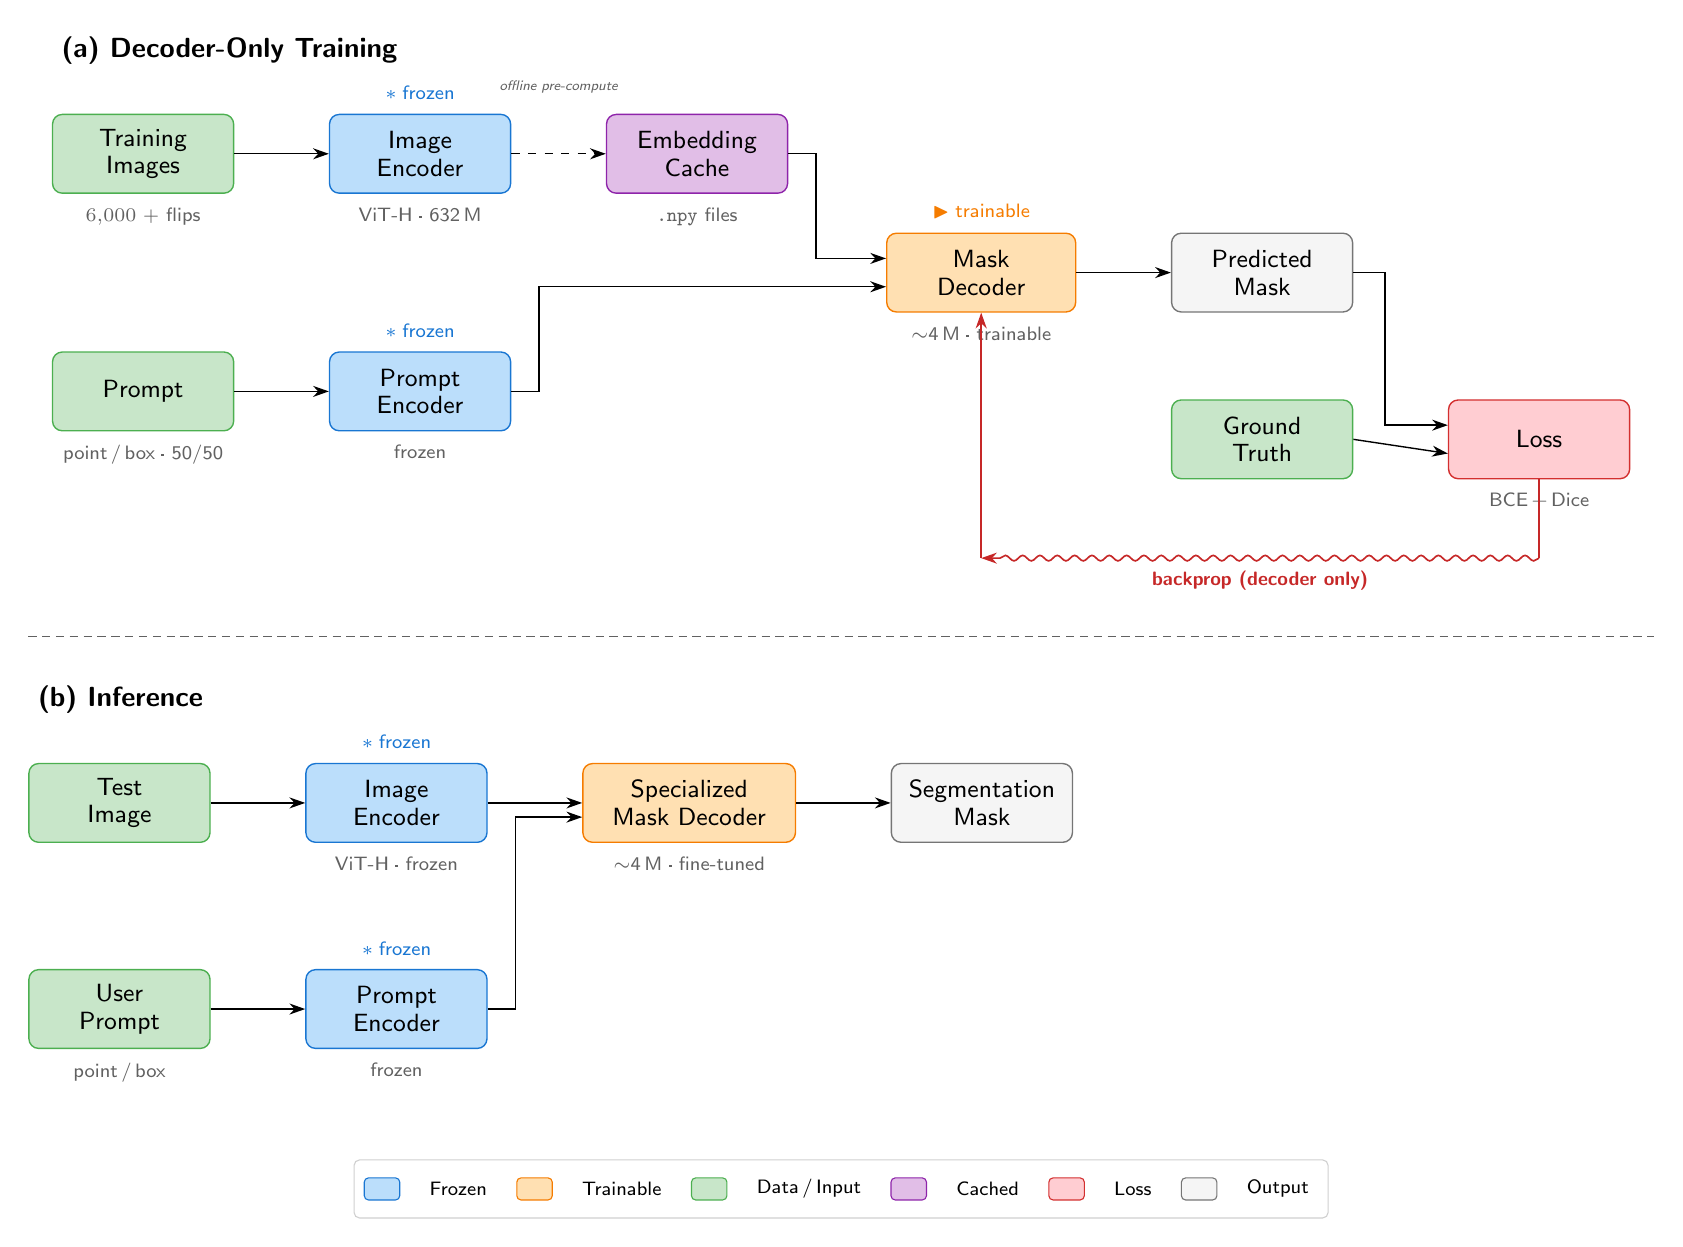
\begin{tikzpicture}[
    nd/.style={rounded corners=3.5pt, minimum height=10mm, minimum width=23mm,
               align=center, font=\small\sffamily, line width=0.5pt},
    ndata/.style  ={nd, fill=cData, draw=cDataB},
    nfrz/.style   ={nd, fill=cFrz,  draw=cFrzB},
    ntrn/.style   ={nd, fill=cTrn,  draw=cTrnB},
    ncch/.style   ={nd, fill=cCch,  draw=cCchB},
    nlos/.style   ={nd, fill=cLoss, draw=cLossB},
    nout/.style   ={nd, fill=cOu,   draw=cOuB},
    ar/.style={-{Stealth[length=2mm,width=1.4mm]}, line width=0.5pt},
    da/.style={ar, dashed},
    sub/.style={font=\scriptsize\sffamily, text=cG, align=center},
    ftag/.style={font=\scriptsize\sffamily, text=cFrzB},
    ttag/.style={font=\scriptsize\sffamily, text=cTrnB},
    ptit/.style={font=\normalsize\bfseries\sffamily, anchor=west},
]

% ======================================================================
%  (a) DECODER-ONLY TRAINING
% ======================================================================
\node[ptit] (tA) at (0,0) {(a) Decoder-Only Training};

% -- ROW 1 : Training Images → Image Encoder  - -→ Embedding Cache -
\node[ndata, below=8mm of tA.west, anchor=north west]
    (img) {Training\\[-1pt]Images};
\node[sub, below=1.5pt of img] {$6{,}000$ + flips};

\node[nfrz, right=12mm of img]
    (enc) {Image\\[-1pt]Encoder};
\node[sub, below=1.5pt of enc]
    {ViT-H\;\textperiodcentered\;632\,M};
\node[ftag, above=1.5pt of enc] {$\ast$\;frozen};

\node[ncch, right=12mm of enc]
    (emb) {Embedding\\[-1pt]Cache};
\node[sub, below=1.5pt of emb] {\texttt{.npy} files};

\draw[ar] (img) -- (enc);
\draw[da] (enc) -- (emb);

\node[sub, font=\tiny\sffamily\itshape,
      above=4pt of $(enc.north east)!0.5!(emb.north west)$]
    {offline pre-compute};

% -- ROW 2 : Prompt → Prompt Encoder ------------------------------
\node[ndata, below=20mm of img]
    (prm) {Prompt};
\node[sub, below=1.5pt of prm]
    {point\,/\,box\;\textperiodcentered\;50/50};

\node[nfrz, right=12mm of prm]
    (pe) {Prompt\\[-1pt]Encoder};
\node[sub, below=1.5pt of pe] {frozen};
\node[ftag, above=1.5pt of pe] {$\ast$\;frozen};

\draw[ar] (prm) -- (pe);

% -- MASK DECODER (centred between rows 1 & 2) --------------------
\coordinate (midY) at ($(emb)!0.5!(pe)$);
\node[ntrn, minimum width=24mm, right=24mm of emb |- midY]
    (dec) {Mask\\[-1pt]Decoder};
\node[sub, below=1.5pt of dec]
    {${\sim}$4\,M\;\textperiodcentered\;trainable};
\node[ttag, above=1.5pt of dec]
    {\raisebox{0.3pt}{$\blacktriangleright$}\;trainable};

% feed-in arrows
\draw[ar] (emb.east) -- ++(3.5mm,0) |- ([yshift=1.8mm]dec.west);
\draw[ar] (pe.east)  -- ++(3.5mm,0) |- ([yshift=-1.8mm]dec.west);

% -- PREDICTED MASK ------------------------------------------------
\node[nout, right=12mm of dec]
    (pred) {Predicted\\[-1pt]Mask};
\draw[ar] (dec) -- (pred);

% -- GROUND TRUTH (below predicted mask) ---------------------------
\node[ndata, below=11mm of pred]
    (gt) {Ground\\[-1pt]Truth};

% -- LOSS (below and between pred & gt, shifted right) -------------
\node[nlos, right=12mm of gt]
    (ls) {Loss};
\node[sub, below=1.5pt of ls] {BCE\,+\,Dice};

\draw[ar] (pred.east) -- ++(4mm,0) |- ([yshift=1.8mm]ls.west);
\draw[ar] (gt.east) -- ([yshift=-1.8mm]ls.west);

% -- BACKPROP (Loss → Decoder) ------------------------------------
% Route: Loss south → down → left → up into decoder south
% Keep the path below Ground Truth so nothing overlaps
\coordinate (bpBot) at ([yshift=-10mm]gt.south);

% The squiggly segment is only the horizontal part
\draw[cBP, line width=0.6pt]
    (ls.south) -- (ls.south |- bpBot);

\draw[ar, cBP, line width=0.6pt,
      decorate, decoration={snake, amplitude=0.35mm, segment length=2.2mm,
                            post length=1.6mm}]
    (ls.south |- bpBot) -- (dec.south |- bpBot);

\draw[cBP, line width=0.6pt, -{Stealth[length=2mm,width=1.4mm]}]
    (dec.south |- bpBot) -- (dec.south);

% backprop label centred on horizontal rail
\node[sub, text=cBP, font=\scriptsize\sffamily\bfseries, anchor=north]
    at ([yshift=-1pt] $(dec.south |- bpBot)!0.5!(ls.south |- bpBot)$)
    {backprop (decoder only)};


% ======================================================================
%  SEPARATOR
% ======================================================================
\coordinate (sepL) at ([xshift=-3mm]img.west);
\coordinate (sepR) at ([xshift=3mm]ls.east);
\coordinate (sepY) at ([yshift=-10mm]bpBot);

\draw[densely dashed, cG, line width=0.4pt]
    (sepL |- sepY) -- (sepR |- sepY);


% ======================================================================
%  (b) INFERENCE
% ======================================================================
\coordinate (tBxy) at ([yshift=-8mm] sepL |- sepY);
\node[ptit] (tB) at (tBxy) {(b) Inference};

% -- ROW 1 : Test Image → Encoder → Decoder → Output
\node[ndata, below=8mm of tB.west, anchor=north west]
    (bi) {Test\\[-1pt]Image};

\node[nfrz, right=12mm of bi]
    (be) {Image\\[-1pt]Encoder};
\node[sub, below=1.5pt of be] {ViT-H\;\textperiodcentered\;frozen};
\node[ftag, above=1.5pt of be] {$\ast$\;frozen};

\node[ntrn, right=12mm of be, minimum width=27mm]
    (bd) {Specialized\\[-1pt]Mask Decoder};
\node[sub, below=1.5pt of bd]
    {${\sim}$4\,M\;\textperiodcentered\;fine-tuned};

\node[nout, right=12mm of bd]
    (bo) {Segmentation\\[-1pt]Mask};

\draw[ar] (bi) -- (be);
\draw[ar] (be) -- (bd);
\draw[ar] (bd) -- (bo);

% -- ROW 2 : User Prompt → Prompt Encoder → Decoder
\node[ndata, below=16mm of bi]
    (bp) {User\\[-1pt]Prompt};
\node[sub, below=1.5pt of bp] {point\,/\,box};

\node[nfrz, right=12mm of bp]
    (bpe) {Prompt\\[-1pt]Encoder};
\node[sub, below=1.5pt of bpe] {frozen};
\node[ftag, above=1.5pt of bpe] {$\ast$\;frozen};

\draw[ar] (bp)  -- (bpe);
% L-shaped route into decoder left side
\draw[ar] (bpe.east) -- ++(3.5mm,0) |- ([yshift=-1.8mm]bd.west);


% ======================================================================
%  LEGEND (single row, centred)
% ======================================================================
\coordinate (legY) at ([yshift=-14mm]bp.south);
\coordinate (legMid) at ($(sepL)!0.5!(sepR)$);
\coordinate (legPos) at (legMid |- legY);

\matrix[anchor=north, column sep=2.5mm, row sep=0pt,
        inner sep=3.5pt,
        nodes={font=\scriptsize\sffamily, anchor=west},
        draw=cG!30, rounded corners=2pt, fill=white]
    at (legPos)
{
    \node[fill=cFrz, draw=cFrzB, rounded corners=1.5pt,
          minimum width=4.5mm, minimum height=2.8mm]{}; &
    \node{Frozen}; &
    \node[fill=cTrn, draw=cTrnB, rounded corners=1.5pt,
          minimum width=4.5mm, minimum height=2.8mm]{}; &
    \node{Trainable}; &
    \node[fill=cData, draw=cDataB, rounded corners=1.5pt,
          minimum width=4.5mm, minimum height=2.8mm]{}; &
    \node{Data\,/\,Input}; &
    \node[fill=cCch, draw=cCchB, rounded corners=1.5pt,
          minimum width=4.5mm, minimum height=2.8mm]{}; &
    \node{Cached}; &
    \node[fill=cLoss, draw=cLossB, rounded corners=1.5pt,
          minimum width=4.5mm, minimum height=2.8mm]{}; &
    \node{Loss}; &
    \node[fill=cOu, draw=cOuB, rounded corners=1.5pt,
          minimum width=4.5mm, minimum height=2.8mm]{}; &
    \node{Output}; \\
};

\end{tikzpicture}
\end{document}
